\chapter{Seiten}

\section{Home}

Die Startseite des ACPs gibt eine allgemeine Schnellerklärung über alle Seiten des ACPs und ist die erste Seite auf der man nach der Anmeldung landet. Neben den allgemeinen Erklärungen stehen auf der Startseite Statistiken und Systeminformationen wie CPU-Auslastung, Laufzeit des Servers, RAM-Nutzung usw.

\begin{figure}[ht]
    \centering
    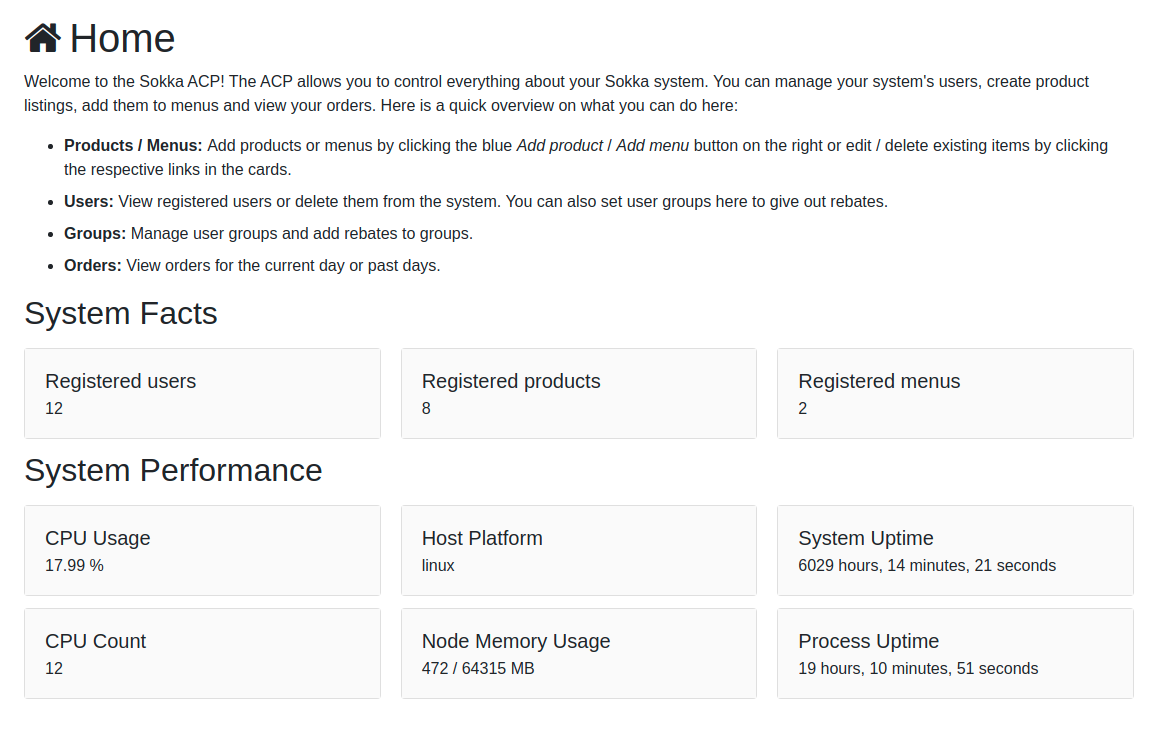
\includegraphics[width=0.8\textwidth]{images/ACP/home.png}
    \caption{Die Startseite des Sokka-ACPs}
\end{figure}

Die Informationen unter \textbf{System Facts} und \textbf{System Performance} aktualisieren sich alle fünf Sekunden automatisch.

\section{Products}

Die Produktseite erlaubt es Produkte im Sokka-System hinzuzufügen, zu bearbeiten und zu löschen.

\begin{figure}[ht]
    \centering
    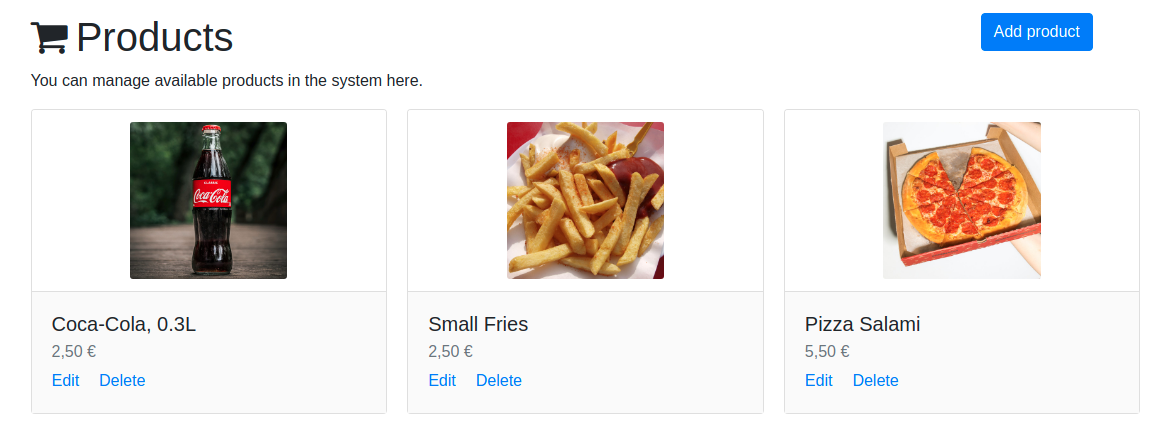
\includegraphics[width=0.8\textwidth]{images/ACP/products.png}
    \caption{Die Produkteseite des Sokka-ACPs}
\end{figure}

\section{Menus}

Die Menüseite erlaubt es Menüs im Sokka-System hinzuzufügen, zu bearbeiten und zu löschen.

\begin{figure}[ht]
    \centering
    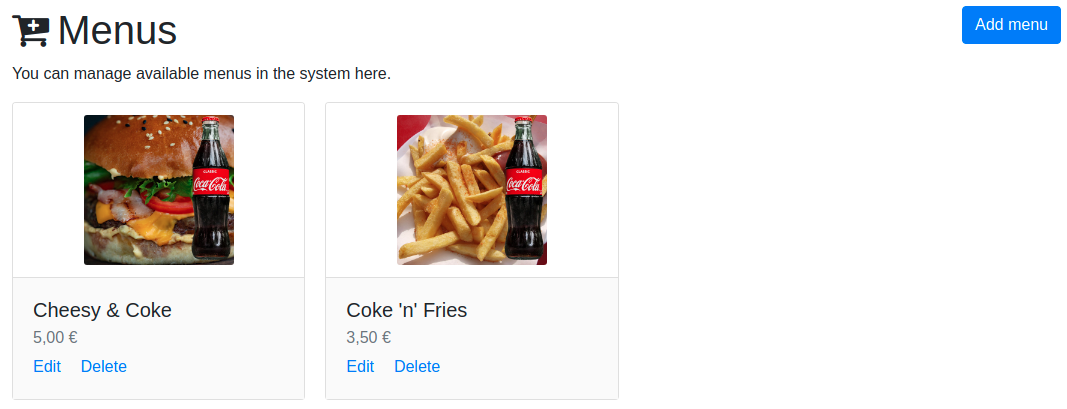
\includegraphics[width=0.8\textwidth]{images/ACP/menus.png}
    \caption{Die Menüsseite des Sokka-ACPs}
\end{figure}

\section{Users}

Die Nutzerseite erlaubt es, registrierten Nutzern im Sokka-System eine Rabattgruppe zuzweisen oder sie komplett aus der Datenbank zu entfernen.

\begin{figure}[ht]
    \centering
    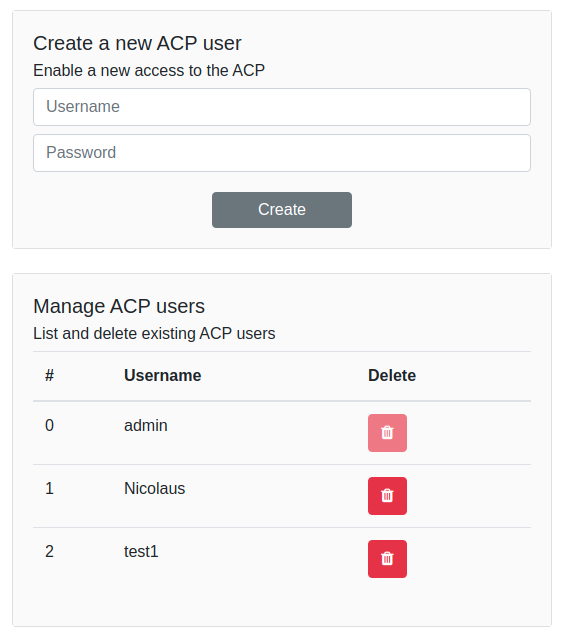
\includegraphics[width=0.8\textwidth]{images/ACP/users.png}
    \caption{Die Nutzerseite des Sokka-ACPs}
\end{figure}

\section{Groups}

Die Gruppenseite erlaubt es, neue Rabattgruppen zu erstellen, existente zu bearbeiten und nicht mehr benötigte zu löschen.

\begin{figure}[ht]
    \centering
    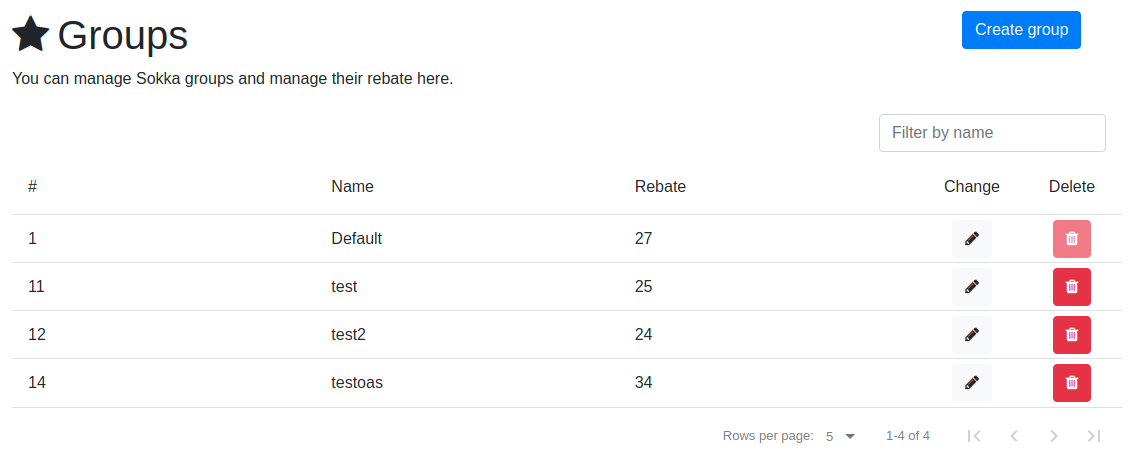
\includegraphics[width=0.8\textwidth]{images/ACP/groups.png}
    \caption{Die Gruppenseite des Sokka-ACPs}
\end{figure}

\section{Orders}

Die Orderseite erlaubt es, getätigte Bestellungen von Nutzern pro Tag einzusehen.

\begin{figure}[ht]
    \centering
    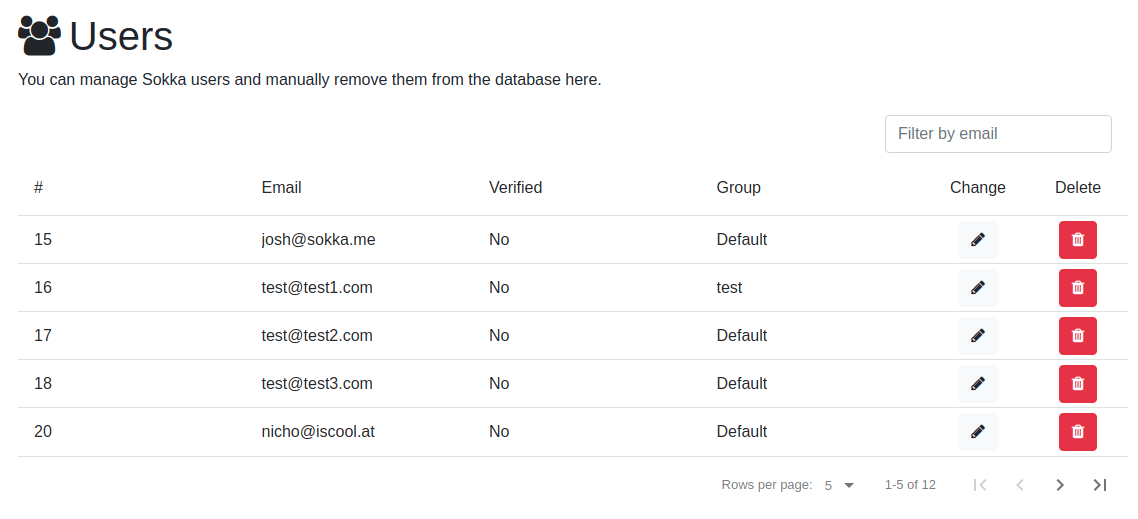
\includegraphics[width=0.8\textwidth]{images/ACP/users-page.png}
    \caption{Die Bestellungsseite des Sokka-ACPs}
\end{figure}

\section{Konfiguration}

Die Konfigurationsseite erlaubt es neben der ACP-Nutzerkontoverwaltung ebenfalls ganz grundlegende Einstellungswerte für das Sokka-System festzulegen, wie beispielsweise die maximal zulässige Bestellzeit des Vortags.

\begin{figure}[ht]
    \centering
    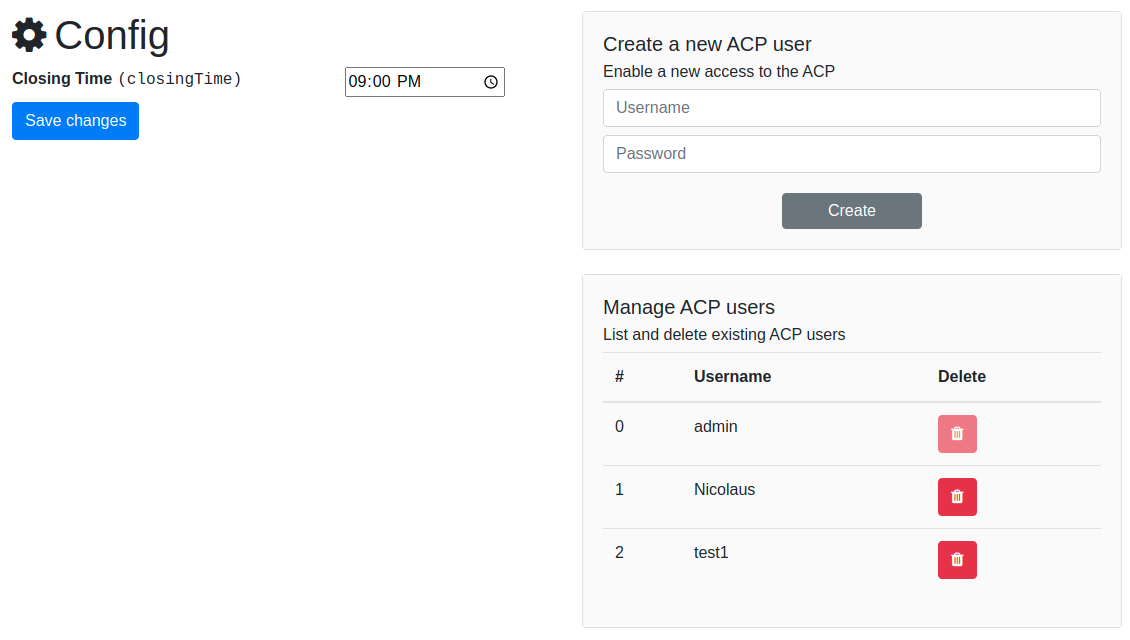
\includegraphics[width=0.8\textwidth]{images/ACP/config.png}
    \caption{Die Konfigurationsseite des Sokka-ACPs}
\end{figure}